% Autor: Leonhard Segger, Alexander Neuwirth
% Datum: 2017-10-30
\documentclass[
	% Papierformat
	a4paper,
	% Schriftgröße (beliebige Größen mit „fontsize=Xpt“)
	12pt,
	% Schreibt die Papiergröße korrekt ins Ausgabedokument
	pagesize,
	% Sprache für z.B. Babel
	ngerman
]{scrartcl}

% Achtung: Die Reihenfolge der Pakete kann (leider) wichtig sein!
% Insbesondere sollten (so wie hier) babel, fontenc und inputenc (in dieser
% Reihenfolge) als Erstes und hyperref und cleveref (Reihenfolge auch hier
% beachten) als Letztes geladen werden!

% Silbentrennung etc.; Sprache wird durch Option bei \documentclass festgelegt
\usepackage{babel}
% Verwendung der Zeichentabelle T1 (Sonderzeichen etc.)
\usepackage[T1]{fontenc}
% Legt die Zeichenkodierung der Eingabedatei fest, z.B. UTF-8
\usepackage[utf8]{inputenc}
% Schriftart
\usepackage{lmodern}
% Zusätzliche Sonderzeichen
\usepackage{textcomp}

% Mathepaket (intlimits: Grenzen über/unter Integralzeichen)
\usepackage[intlimits]{amsmath}
% Ermöglicht die Nutzung von \SI{Zahl}{Einheit} u.a.
\usepackage{siunitx}
% Zum flexiblen Einbinden von Grafiken (\includegraphics)
\usepackage{graphicx}
% Abbildungen im Fließtext
\usepackage{wrapfig}
% Abbildungen nebeneinander (subfigure, subtable)
\usepackage{subcaption}
% Funktionen für Anführungszeichen
\usepackage{csquotes} 
\MakeOuterQuote{"}
% Zitieren, Bibliographie
\usepackage{biblatex}


% Zur Darstellung von Webadressen
\usepackage{url}
%chemische Formeln
\usepackage[version=4]{mhchem}
% siunitx: Deutsche Ausgabe, Messfehler getrennt mit ± ausgeben
\usepackage{floatrow}
\floatsetup[table]{capposition=top}
\usepackage{float}
% Verlinkt Textstellen im PDF-Dokument
\usepackage[unicode]{hyperref}
% "Schlaue" Referenzen (nach hyperref laden!)
\usepackage{cleveref}
\sisetup{
	locale=DE,
	separate-uncertainty
}
\bibliography{14Mo_W1_14-05-2018_References}

\begin{document}
	
	\begin{titlepage}
		\centering
		{\scshape\LARGE Versuchsbericht zu \par}
		\vspace{1cm}
		{\scshape\huge W1 - Stirling-Motor \par} 
		\vspace{2.5cm}
		{\LARGE Gruppe 14Mo \par}
		\vspace{0.5cm}
		
		{\large Alexander Neuwirth (E-Mail: a\_neuw01@wwu.de) \par}
		{\large Leonhard Segger (E-Mail: l\_segg03@uni-muenster.de) \par}
		\vfill
		
		durchgeführt am 14.05.2018\par 
		betreut von\par
		{\large Torsten Stiehm} 
		
		\vfill
		
		{\large \today\par}
	\end{titlepage}
	\tableofcontents
	\newpage

	\section{Kurzfassung}
	%TODO Hypothese	und deren Ergebnis, wenn Hypothese ist, dass nur Theorie erfüllt, sagen: Erwartung: Theorie aus einführung (mit reflink) erfüllt
	%TODO Ergebnisse, auch Zahlen, mindestens wenn's halbwegs Sinn ergibt
	%TODO Was wurde gemacht
	%TODO manche leute wollen Passiv oder "man", manche nicht
	Es wurde der Stirling-Motor als Wärmepumpe und als Kältemaschine untersucht.
	Konkret wurde der Gefrier- und Schmelzvorgang einer geringen Menge Wasser durch die Heiz- bzw. Kühlleistung des Stirlingmotors betrachtet.
	Dazu konnte zunächst die Reibungswärme, die innerhalb des Motors auftritt und mit dem Kühlwasser abtransportiert wird, bestimmt werden, um sie in den folgenden Betrachtungen abziehen zu können.
	Dann wurde aus dem Temperaturverlauf in Abhängigkeit von der Zeit und der Betriebsrichtung des Stirling-Motors die Heiz- und Kühlleistung sowie die Leistungszahl des Motors als Kältemaschine bzw. Wärmemaschine bestimmt und verglichen.
	Außerdem wurden die Schmelzwärme und spezifische Wärme von Wasser bestimmt.
	Es wurde angenommen, dass die Verwendung eines Stirling-Motors eine geeignete Methode ist diese Werte zu bestimmten.
	Da die Literaturwerte die Messwerte von Schmelzwärme von Wasser $S$ = \SI{233,7\pm 4,5}{J/g} und spezifischer Wärme von Eis $c_\text{Eis}$ = $\SI{2,254+-0,007}{J/g/K}$ nicht hinreichend präzise bestätigten, konnte diese Annahme nicht bestätigt werden.%TODO soll ich lit.-Wert erwähnen?
	
	\section{Methoden} \label{sec_Methoden}
	
	In \cref{Aufbau} ist der verwendete Stirling-Motor dargestellt.
	Zunächst wurden die Verluste durch Reibung bestimmt.
	Dazu wurde der Motor mit offenem Zylinderkopf betrieben, sodass der Druck im Zylinder konstant bei Luftdruck lag und abgesehen von Reibungswärme keine Heiz- oder Kühlwirkung entstehen konnte.
	Bei diesem Betrieb wurde dann zunächst der Volumendurchsatz des Kühlwassers bestimmt, indem an der Pumpe mit Stoppuhr und Messzylinder die Zeit und der Füllstand nach ca. \SI{9}{\second} gemessen.
	Dies wurde fünf mal durchgeführt, um den den Mittelwert bilden und den Messfehler verringern zu können.
	Dann wurde die Temperaturerhöhung des aus dem Motor abfließenden Wassers gegenüber dem Wasser im Tank, der die Pumpe speist, gemessen.
	Für diese und die folgenden Messungen wurde für die Drehzahl des Elektromotors etwa \SI{3}{\kilo \hertz} gewählt.
	Gemessen wurde die Frequenz, indem eine Fouriertransformation durchgeführt wurde und die Spitze dieser betrachtet wurde.
	
	Im zweiten Teil wurde ein Reagenzglas mit ca. \SI{1}{\milli \liter} Wasser (mit einer Pipette befüllt) in den Zylinderkopf eingesetzt und dieser geschlossen.
	Dann wurde bei gleicher Umlaufrichtung (als Kältemaschine) die Temperatur im Reagenzglas in Abhängigkeit von der Zeit gemessen und am Ende wie zuvor der Temperaturunterschied zwischen abfließendem Kühlwasser und Wassertank gemessen.
	
	Sobald ca. \SI{-25}{\degreeCelsius} erreicht waren, wurde die Umlaufrichtung des Elektromotors geändert, sodass der Stirling-Motor als Wärmepumpe fungierte und erneut die Temperatur im Reagenzglas in Abhängigkeit von der Zeit gemessen.
	Auch hier wurde am Ende der Temperaturunterschied des Kühlwassers gemessen.
	
	\begin{figure}[H]
		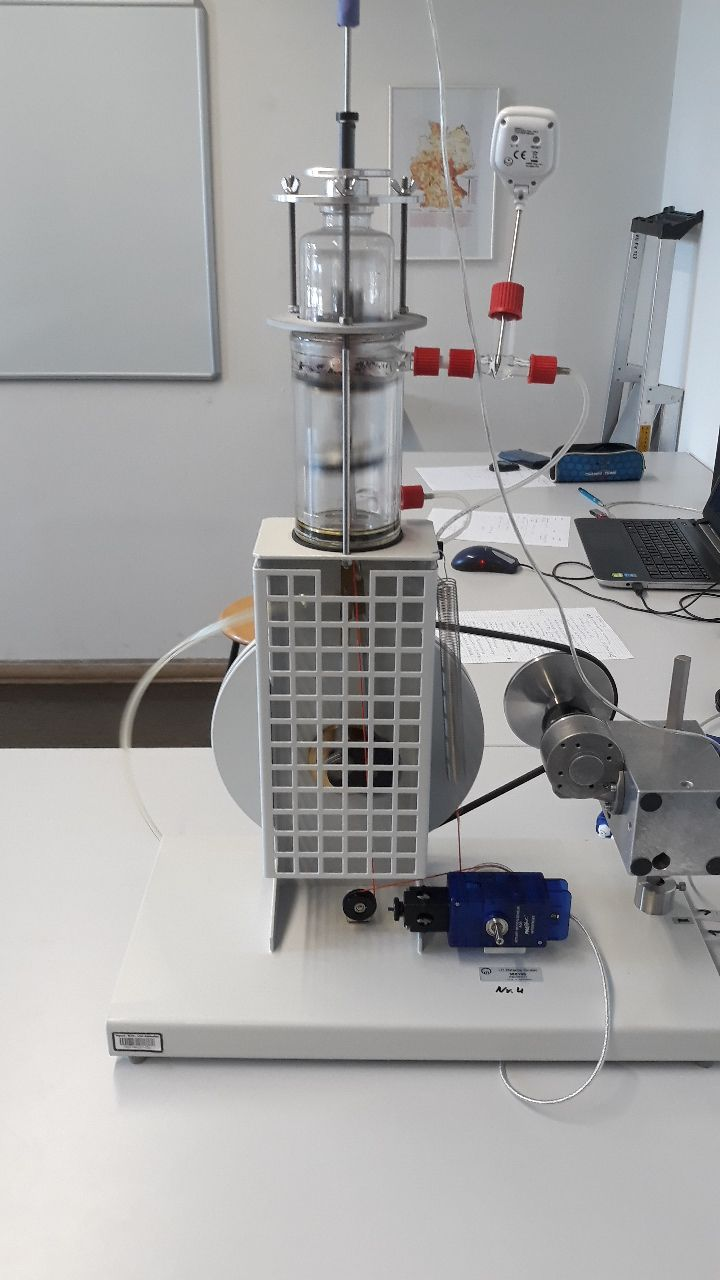
\includegraphics[width=0.29\textwidth]{Aufbau}
		\centering
		\caption{Aufbau des Stirling-Motors.}
		\label{Aufbau}
		\centering
	\end{figure} 

	\section{Ergebnisse und Diskussion}
	%TODO Unsicherheiten
	

	\subsection{Beobachtung und Datenanalyse}
	
	\subsubsection{Unsicherheiten} 
	Die Unsicherheiten wurden gemäß GUM ermittelt. 
	Außerdem wurde für Unsicherheitsrechnungen die Python Bibliothek "uncertainties" verwendet.
	\begin{description}
		\item[Messzylinder] Die Unsicherheit des Messzylinders wurde mit \SI{0,04}{mL} abgeschätzt (dreieckige WDF).
		\item[Stoppuhr] Die Stoppuhr zeigt Sekunden mit Zwei Nachkommastellen an, woraus eine Unsicherheit von \SI{0,004}{s} folgt (rechteckige WDF), jedoch hat die Reaktionszeit einen größeren Einfluss, wesshalb eine Unsicherheit von \SI{0,1}{s} angenommen wird. 
		\item[Pipette] Auf der Pipette, die zum Füllen des Reagenzglases m Zylinderkopf verwendet wurde, ist eine Unsicherheit von \SI{0,007}{mL} angegeben.
		\item[Thermometer] Die Unsicherheit des Kühlwasserthermometers vom Typ K ist \SI{1,5}{\degreeCelsius} in dem gemessenen Temperaturintervall. Da eine derartig große Unsicherheit keine Aussage zulassen würde, nehmen wir an, dass dies im Wesentlichen ein systematischer Fehler ist, der  für das Messen von Temperaturdifferenzen kaum Einfluss hat und schätzen die Unsicherheit der Temperaturdifferenz aufgrund der Schwankungen der Thermometeranzeige mit \SI{0,05}{\degreeCelsius} ab. %TODO approven
		\item[Motorfrequenz] Die Unsicherheit der durch Fouriertransformation ermittelten Frequenzen wurde mit \SI{0,01}{Hz} abgeschätzt, da die Frequenz kaum schwankte und keine anderen Frequenzen im Frequenzbild auftraten.
	
	\end{description}
	\subsubsection{Bestimmung der Reibungsverluste}
	Die Reibungsverluste lassen sich aus der Erwärmung des Kühlwassers beim Betrieb der Wärmepumpe bzw. Kältemaschine bei offenem Zylinderkopf bestimmen.
	Die zugeführte Wärmemenge $\Delta{Q}$ ist proportional zur Temperaturänderung $\Delta{T}$:
	\begin{equation}
	\Delta{Q} = C_W \cdot \Delta{T} = c \cdot m \cdot \Delta{T}
	\label{eq_Wärme}
	\end{equation} 
	Für Wasser beträgt die spezifische Wärme $c_{H_2O}$ = \SI{4,185}{J/g/K}. %Heslig, aber tut nicht anders
	Die Masse $m$ der Gesamtwassermenge im System ist nicht direkt bestimmbar, der Durchfluss des Kühlwassers $d=m/t$ hingegen schon.
	Somit lässt sich mit \cref{eq_Wärme} die an das Kühlwasser abgegebenen Leistung $\Delta{Q}/t$ ermitteln.
	Die gesuchte Reibungsarbeit pro Umlauf erhält man durch Division der Leistung durch die Frequenz des Motors.
	Es folgt:
	\begin{equation}
	W_R = c_{H_2O} \cdot \frac{d}{f} \cdot \Delta{T} %TODO \text{R} weil von Wort?
	\label{eq_Reibungsarbeit}
	\end{equation}
	Der Durchfluss $d$ ergibt sich indem man die geflossene Wassermenge $v$ durch die gestoppte Zeit $t$ dividiert und mit der Dichte $\rho_{H_2O}$ multipliziert. Aus \cref{tab_Durchfluss} ergibt sich ein Mittelwert von \SI{4,61+-0,13}{mL/s} und somit ein Durchfluss $d$ = \SI{4,61+-0,13}{g/s}.
	
	Die Frequenz des Motors wurde mittels FFT auf \SI{3,15+-0,01}{Hz} eingestellt (vgl. \cref{sec_Methoden}).
	Die Temperaturänderung des Kühlwassers $\Delta{T}$ betrug \SI{0,5+-0,05}{\degreeCelsius}.
	Es folgt eine Reibungsarbeit pro Umlauf gemäß \cref{eq_Reibungsarbeit} von $W_R=\SI{2,76+-0,29}{J}$.
	\begin{table}[H]
		\centering
		\begin{tabular}{ c | c }
			Wassermenge $v$ in \SI{}{mL} & Zeit $t$ in \SI{}{s} \\ \hline
			\SI{38,0+-0,03}{}&\SI{8,16+-0,1}{}\\
			\SI{40,8+-0,03}{}&\SI{8,50+-0,1}{}\\
			\SI{41,4+-0,03}{}&\SI{9,34+-0,1}{}\\
			\SI{49,2+-0,03}{}&\SI{10,78+-0,1}{}\\
			\SI{47,0+-0,03}{}&\SI{10,22+-0,1}{}\\
		\end{tabular}
		\caption{Gemessene Kühlwassermenge die durch den Stirling-Motor in einer bestimmten Zeit fließt.}
		\label{tab_Durchfluss} 
	\end{table}
	
	\subsubsection{Bestimmung der Kühlleistung} \label{sssec_Kühlleistung}
	Die pro Umlauf aufzuwendende mechanische Arbeit $-W$ ist durch
	\begin{equation}
	W =  Q_1 - Q_2 + W_R
	\end{equation}
	gegeben.
	Die Wärme $Q_2$ wird dem Zylinderkopf pro Umlauf entzogen und die Wärme $-Q_1$ wird dem Kühlwasser zu geführt.
	
	$Q_1+W_R$ lässt sich analog zur Reibungsarbeit pro Umlauf mit \cref{eq_Reibungsarbeit} bestimmen.	
	Die gemessene Temperaturänderung des Kühlwassers betrug $\Delta{T}$=$\SI{1,0+-0,05}{\degreeCelsius}$ woraus $Q_1+W_R$=$\SI{5,53+-0,33}{J}$ folgt.
	
	$Q_2$ ergibt sich aus der Steigung der Messkurve in \cref{fig_Kuehl}.
	Es wurde ein linearer Fit verwendet, um die Steigung $s$ nahe der Raumtemperatur zu bestimmen.
	Die Kühlleistung $P_\text{Kühl}$ ist gegeben durch zeitliches Ableiten von \cref{eq_Wärme}.
	\begin{equation}
	\dot{Q} = P_\text{Kühl} = c \cdot m \cdot s = c \cdot \rho \cdot V \cdot s 
	\label{eq_Kühlleistung}
	\end{equation}
	
	Mittels Division der Kühlleistung $P_\text{Kühl}$ durch die Frequenz des Motors erhält man die Wärme $Q_2$ pro Umlauf:
	\begin{equation}
	Q_2 = \frac{P_\text{Kühl}}{f} = c \cdot \rho \cdot V \cdot \frac{s}{f}	
	\end{equation}
	In dem Reagenzglas im Zylinderkopf befand sich $V$=\SI{1+- 0,007}{mL} destilliertes Wasser und die Steigung $s$ beträgt $\SI{0,2002+-0,0002}{\degreeCelsius/s}$. %TODO Satz
	Folglich ist $P_\text{Kühl}$ = \SI{0,838+-0,006}{W} und $Q_2$ = $\SI{0,266+-0,002}{J}$.
	
	Die Leistungszahl $\epsilon$ ist der Quotient der entnommenen Wärmemenge $Q_2$ und aufgewandter Arbeit $W$:
	\begin{equation}
		\epsilon = \frac{|Q_2|}{|W|}
		\label{eq_Leistungszahl}
	\end{equation}
	Hier beträgt $W=Q_1+W_R-Q_2=\SI{5,26+-0,33}{J}$ woraus eine Leistungszahl von $\epsilon$ = $\SI{5,1 +- 0,3}{\%}$ folgt.
	
	\begin{figure}[H]
		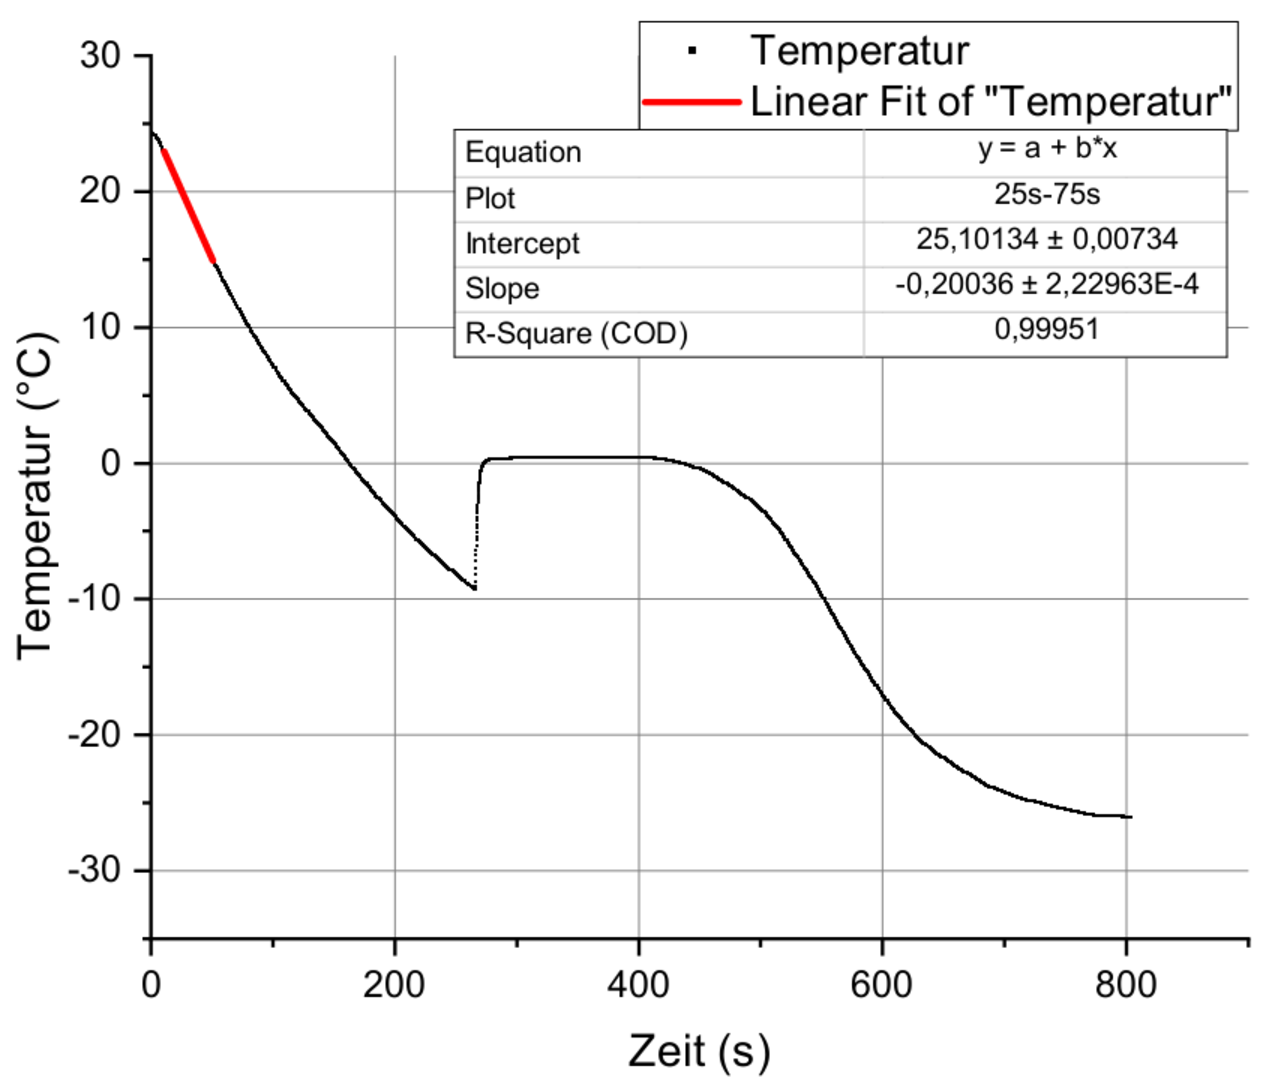
\includegraphics[width=0.7\textwidth]{Kuehl}
		\centering
		\caption{Gemessene Temperatur als Funktion der Zeit beim Betrieb des Stirling-Motors als Kältemaschine. Die Fehler sind kleiner als die Symbolgröße.}
		\label{fig_Kuehl}
		\centering
	\end{figure}

	Unter der Annahme, dass der Motor der Probe konstant Wärme entzieht, lässt sich die von dem Wasser beim Schmelzen abgegebene Wärme anhand von \cref{fig_Kuehl} abschätzen. %TODO wat???????? Da schmilzt nichts...!!
	Im Zeitraum von \SI{266+-2}{s} bis \SI{545+-5}{s} entzieht der Motor dem Wasser Wärme, die Anfangs- und Endtemperatur sind jedoch gleich. 
	Folglich entspricht die entzogene Wärme pro Masse der Schmelzwärme $S$ = \SI{233,7+-4.5}{J/g}, gemäß:
	\begin{equation}
	S = \frac{Q}{m} = c \cdot s\cdot \Delta{t}
	\end{equation}
	
	
	
	\subsubsection{Bestimmung der Heizleistung}
	Die Heizleistung lässt sich analog zur Kühlleistung in \cref{sssec_Kühlleistung} aus der Steigung $s_l$ der Messkurve bei Raumtemperatur in \cref{fig_Waerm} bestimmen. %TODO soll das ein anderes s_l sein als danach? Ich glaub nicht, deshalb mach das pls auch nicht anders...!!
	
	Die Steigung $s_\text{l}$ beträgt \SI{0,377+-0,001}{\degreeCelsius/s} somit folgt aus \cref{eq_Kühlleistung} eine Heizleistung $P_\text{Heiz}$ von \SI{1,58+-0,01}{W}.
	%TODO CHECK START
	Analog lässt sich auch die Leistungszahl $\epsilon$ bestimmen. 
	Die Temperaturänderung $\Delta{T}$ betrug $\SI{0,3+-0,05}{\degreeCelsius}$ woraus gemäß \cref{eq_Reibungsarbeit} ein $Q_1+W_R$ von $\SI{1,66+-0,28}{J}$ folgt. 
	$Q_2$ ergibts sich aus $P_\text{Heiz}/f$=\SI{0,501+-0,004}{J}. %TODO CREFS auf gleichungen
	Die Leistungszahl beträgt somit \SI{43,1+-10,4}{\%}.
	\begin{figure}[H]
		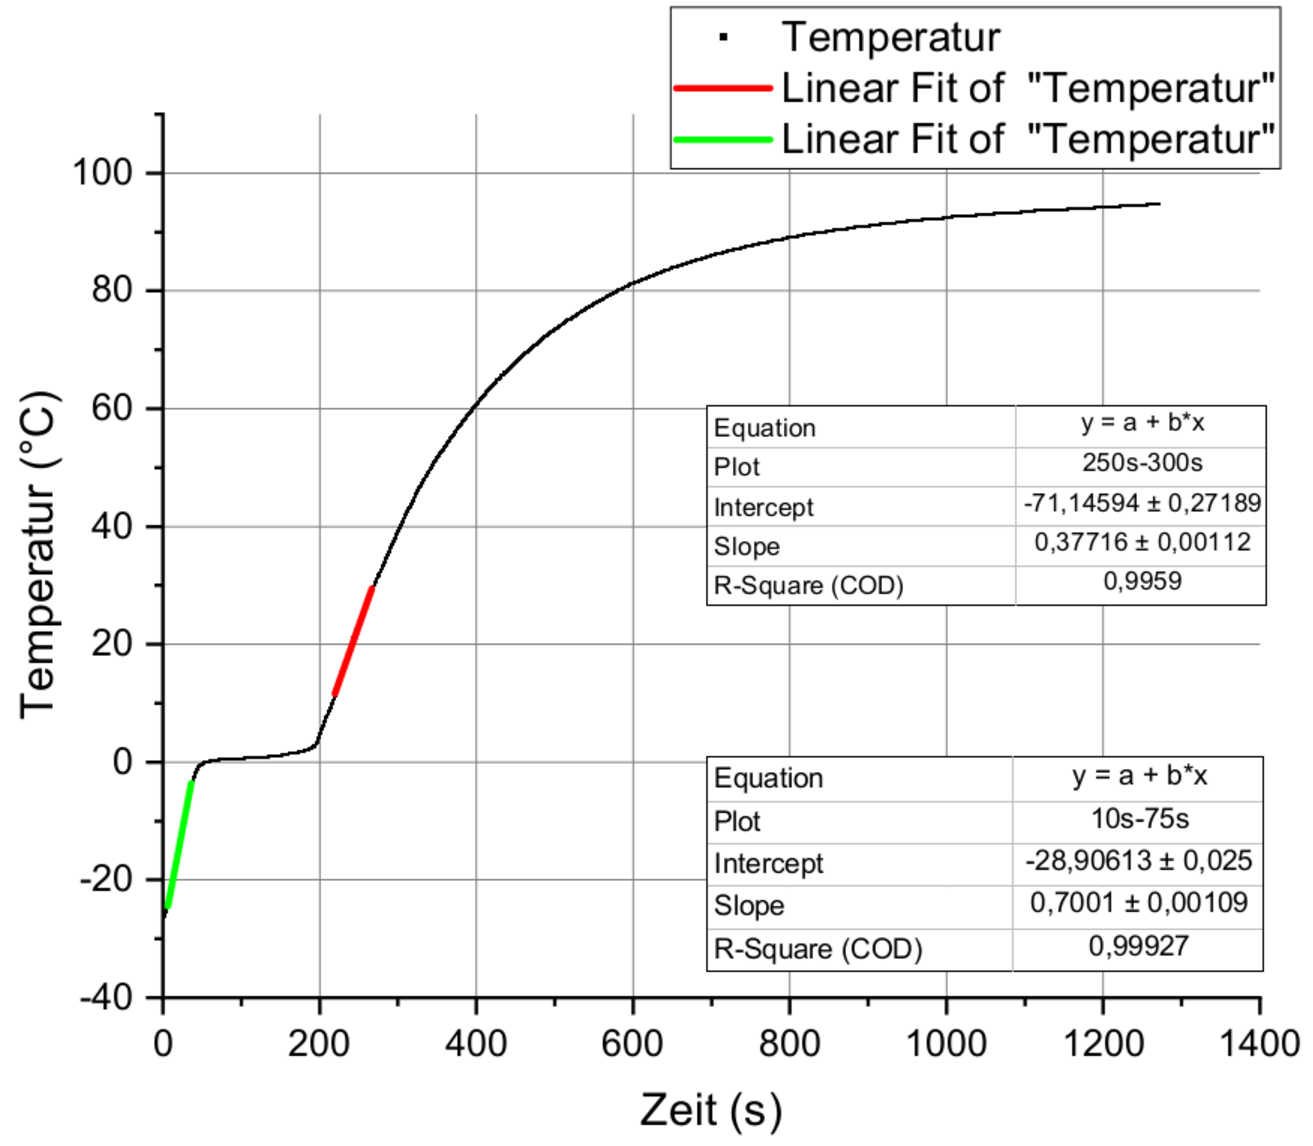
\includegraphics[width=0.7\textwidth]{Waerm}
		\centering
		\caption{Gemessene Temperatur als Funktion der Zeit beim Betrieb des Stirling-Motors als Wärmepumpe. Die Fehler sind kleiner als die Symbolgröße.}
		\label{fig_Waerm}
		\centering
	\end{figure}
	%TODO CEHCK END
	Die spezifische Wärme von Eis lässt sich aus \cref{eq_Kühlleistung} bestimmen:
	\begin{equation}
		c_\text{Eis} = \frac{P_\text{Heiz}}{m \cdot s_\text{s}} = c_{H_2O} \frac{s_\text{l}}{s_\text{s}}
	\end{equation} 
	Die Steigung $s_\text{s}$ nimmt einen Wert von \SI{0,700+-0,001}{\degreeCelsius/s} im Bereich von \SI{-25}{\degreeCelsius} bis \SI{-5}{\degreeCelsius} an. 
	Es ergibt sich eine spezifische Wärme für Eis $c_\text{Eis}$ von $\SI{2,254+-0,007}{J/g/K}$.
	\subsection{Diskussion}
	
	Der abrupte Sprung in \cref{fig_Kuehl} kommt durch die Natur des Kristallisationsprozesses zustande:
	Bei Raumtemperatur ist das destillierte Wasser eine ungesättigte Lösung, da trotz der Destillation kleine Mengen an Salzen im Wasser gelöst sind.
	Wenn nun das Wasser abgekühlt wird, sinkt die Menge an Salzen, die eine gesättigte Lösung ergeben würden, bis sie geringer als die tatsächlich im Wasser enthaltene Menge an Salzen ist, also eine übersättigte Lösung vorliegt.
	An diesem Punkt reicht eine leichte Störung des Systems durch äußere Einflüsse wie die Schwingungen, die der Elektromotor verursacht, um den Salzen ein Anordnen um Kristallisationskeimen zu ermöglichen.
	Um diesen Keim herum kann dann die gesamte Lösung (hier Wasser) lawinenartig kristallisieren.
	
	Das darauf folgende Intervall ohne Temperaturänderung lässt sich dadurch begrünen, dass hier die Wärme, die dem Wasser entzogen wird sich nicht mehr in einen Temperaturunterschied überträgt, sondern die Kristallisation des Wassers zufolge hat.
	Erst sobald der Großteil des Wassers fest ist, führt der Wärmeentzug wieder zu einer Temperaturänderung.
	
	Analog ist das Intervall ohne Temperaturänderung in \cref{fig_Waerm} zu erklären, da hier die dem Eis zugeführte Wärme nicht eine Temperaturänderung bewirkt, sondern die Kristallstruktur des Wassers auflöst und es schmilzt.
	
	In \cref{fig_Waerm} ist außerdem zu erkennen, dass der Temperaturanstieg abnimmt, je näher die Probe an die Siedetemperatur kommt.
	Dies hängt einerseits mit der Abgabe von Wärme an die Umgebung und andererseits mit der stochastischen Natur des Phasenübergangs vom flüssigen in den Gasförmigen Zustand zusammen.
	Hier wird ein zunehmender Anteil der zugeführten Wärme aufgewandt, um diesen Phasenübergang zu ermöglichen und Teile der Probe verdampfen.
	
	Für die Schmelzwärme von Wasser wurde ein Messwert von \SI{233,7\pm 4,5}{J/g} ermittelt.
	Der Literaturwert \cite{schmelzWarm} von \SI{334}{J/g} liegt weit oberhalb Unsicherheiten dieses Messwerts.
	Dies hängt vermutlich damit zusammen, dass beim Betrieb als Kältemaschine die Wasserprobe, während ihr Wärme entzogen wird, Wärme aus der Umgebung des Motors aufnehmen kann.
	Dies ließ sich darin beobachten, dass zunächst Wasser am Zylinder kondensierte und dann kristallisierte und erklärt auch den gekrümmten Verlauf von \cref{fig_Kuehl} vor der Kristallisation.
	
	Die Literatur \cite{spezWarm} gibt für die spezifische Wärme von Eis bei \SI{-10}{\degreeCelsius}einen Wert von \SI{2,220}{J/g/K} an.
	Dies liegt nah an dem Messwert von \SI{2,254\pm 0,007}{J/g/K}, aber nur innerhalb der fünffachen Unsicherheit.
	Dies hängt vermutlich damit zusammen, dass die spezifische Wärme temperaturabhängig ist und der Literaturwert keine Unsicherheit hat. %TODO approven pls
	Insofern kann die Möglichkeit der Verwendung eines Stirling-Motors zur Bestimmung der Schmelzwärme und spezifischen Wärme nicht bestätigt werden.
	
	Wenn man die Leistungszahlen des Stirling-Motors als Wärmepumpe (\SI{43,1+-10,4}{\%}) und als Kältemaschine (\SI{5,1 +- 0,3}{\%}) vergleicht, stellt man fest, dass erstere deutlich höher ist.
	Das kann ebenfalls damit zusammenhängen, dass beim Betrieb als Kältemaschine das Wasser Wärme aus der Umgebung aufgenommen hat.
	Andersherum konnte dies beim Betrieb als Wärmepumpe nicht so stark stattfinden, da die Umgebungsluft bereits gasförmig war und die Energie nicht für eine Änderung des Aggregatzustands verwenden konnte und somit die Energie durch Konvektion und Wärmeleitung durch mechanische Kopplung abtransportiert werden musste.
	
	\section{Schlussfolgerung}
	%TODO Rückgriff auf Hypothese und drittes Nennen dieser
	Es konnte der verwendete Stirling-Motor auf seine Eigenschaften als Wärmepumpe und als Kältemaschine untersucht werden.
	Dazu gehört die Bestimmung der Heiz- bzw. Kühlleistung sowie der Leistungszahlen beider Betriebsmodi.
	Auch konnte gezeigt werden, dass der Stirling-Motor keine geeignete Methode zur präzisen Bestimmung der Schmelzwärme und spezifischen Wärme von Wasser ist.
	Für einen Stirling-Motor mit höheren Leistungszahlen und einer präziseren Bestimmung der Schmelzwärme wäre eine bessere Isolation des Motors von der Umwelt nötig.
	\printbibliography
\end{document}
